\chapter{Implementierung}

Die Architektur des CTGameStudio in der Erstversion musste angepasst werden, um den Anforderungen
des neuen Spielmodus zu erfüllen. Das Hinzufügen eines zweiten Roboters erfordert, mehrere Instanzen
der blockly-Komponente und des Strategie-Interpreters zu erzeugen. Die gleichzeitige Ausführung
mehrerer Strategien musste ermöglicht werden. Die Gameloop und Roboterspielobjekte mussten so angepasst werden, dass die Roboter sinnvoll miteinander interagieren und sich so verhalten, dass ein
gut nachverfolgbares Gameplay möglich ist und unterschiedliche Strategieansätze zum Erfolg führen.
Das Spiel musste um Dialoge mit Formularelementen und Turniervisualisationen erweitert werden. Zur
Persistenz und Interaktion zwischen verschiednen Benutzern des Systems muss das System das Speichern
und Laden von Daten über HTTP-Schnittstellen des Servers unterstützen.

\section{Architektur der Erstversion}

Das ctGameStudio ist ein Webanwendung. Der Server liefert Seiten an den Browser aus und bietet
Login-Management. Unterstützt wird dies durch das auf Node.JS und MongoDB basiertem
KeystoneJS-Framework \footnote{https://keystonejs.com}. Die Darstellung und das dynamische Verhalten
des Spiels basiert auf browser-seitig ausgeführtem HTML und CSS, und Javascript (Abb.
\ref{architektur-alt}). Neben Standard-HTML-Inputs wird Phaser \footnote{https://phaser.io} genutzt,
um mittels WebGL Spielelemente zu rendern.

\begin{figure}
  \caption{Architektur des ctGameStudio in der Erstversion.
  Phaser-Spielobjekte sind rot hervorgehoben. Durchgezogene Linien zeigen
  Beziehungen zwischen Komponenten und Subkomponenten, wobei die Komponente die
  Subkomponente erstellt, besitzt, oder einbindet. Gestrichelte Linien zwischen
  Komponenten zeigen Abhängigkeiten, so dass eine Komponente die andere
  referenziert und den internenen Zustand der Komponente verändert.}

  \label{architektur-alt}
  
  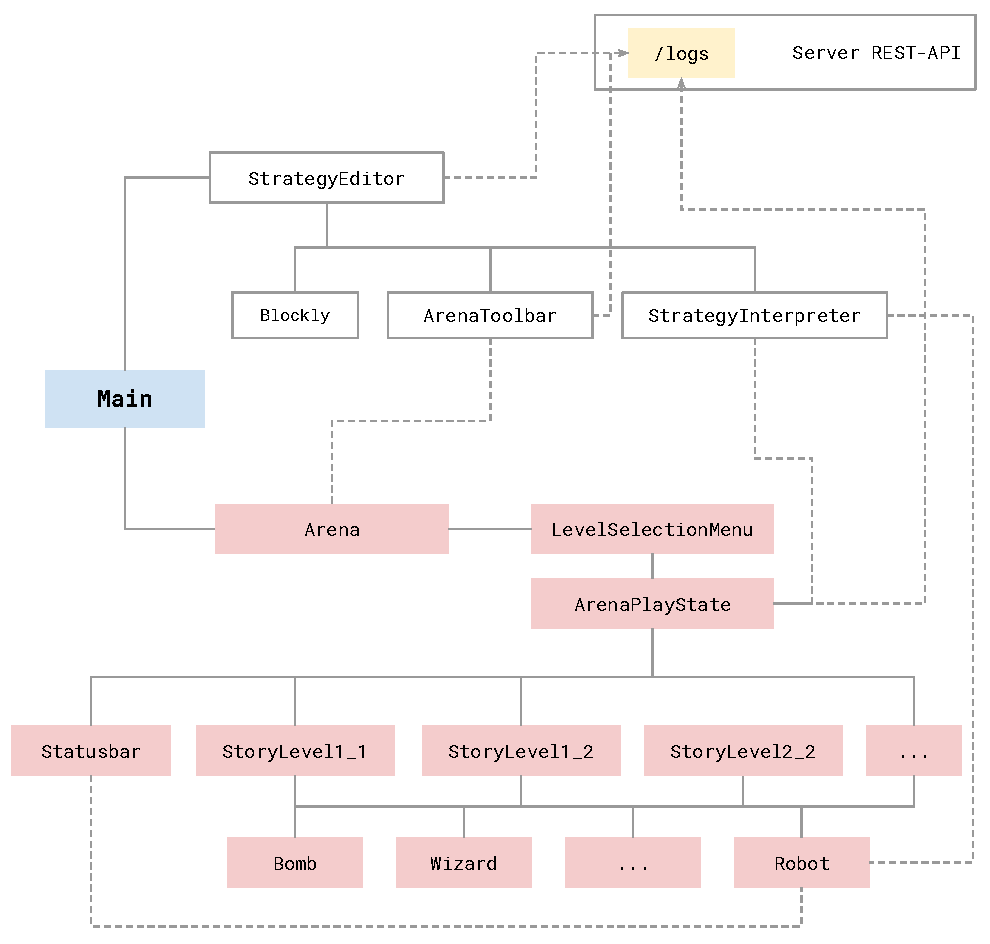
\includegraphics{figures/architektur-alt.pdf}
\end{figure}

Komponenten sind als als Javascript-Funktionen, Objekte oder Klassen definiert. Während eine
Strukturierung dadurch erfolgt, dass Komponenten auf mehrere Dateien aufgeteilt sind, liegen die
Komponenten, Instanzen der Komponenten als auch interne Zustandsvariablen in einem globalen
Namensraum. Dadurch ist direkter Zugriff von eigentlich unabhängigen Komponenten aufeinander möglich
und führt zu einer hohen Kopplung zwischen Komponenten.

\subsection{Main}

Die Hauptfunktion wird nach Laden der Webseite aufgerufen und inialisiert das Phaser-Spiel, welches
das Spielmenü und die Roboter-Umgebung enthält, sowie den Strategieeditor.

\subsection{Strategieeditor}

Der Strategieeditor enthält den Blockly-Oberfläche zur Erstellung eines Programms, den
Strategieinterpreter der für die Ausführung der Strategie zuständig ist, und eine Toolbar mit
Steuerungselemente zur Ausführung der Strategien und Aufruf des Blocklexikons.

\subsection{Blockly}

Die Blockly\footnote{https://developers.google.com/blockly/}-Bibliothek stellt einen Editor zur
blockbasierten Programmierung bereit. Zur Konfiguration des Editors werden die Blöcke definiert, aus
denen der Anwender sein Programm zusammenstellen kann. Die Konfiguration besteht aus einer
Beschreibung der Blöcke sowie aus Funktionen, die beschreiben, welcher Code aus einem Block
generiert werden soll (Abb. \ref{block-configuration}). Die
Blockly-Developer-Tools\footnote{https://blockly-demo.appspot.com/static/demos/blockfactory/index.html}
können genutzt werden, um die Block-Konfiguration zu generieren und zu verwalten.

Für das ctGameStudio wurden Blöcke definiert, die Aktionen des Roboters entsprechen. Der aus einem
Block generierte Code ist ein Funktionsaufruf, der im Aufruf einer Methode des Roboter-Spielobjekts
resultiert (z.B. Abb. \ref{block-configuration}, Zeile 18).

\begin{figure}
  \caption{Konfiguration eines Blocks}

  \label{block-configuration}

  \begin{lstlisting}
    // Beschreibung des Blocks
    Blockly.Blocks.turn = {
      init() {
        this
          .appendField('drehen nach')
          .appendField(new Blockly.FieldDropdown([
            ['rechts', 1], ['links', -1]
          ]), 'direction')
          .appendField('um')
          .appendField('rechts')
          .appendValueInput('angle')
        this.setTooltip(
         `Roboter dreht sich um einen bestimmten Winkel`
         `in angegebener Richtung`
        );
      }
    }

    // Generierung des Codes
    Blockly.JavaScript.turn = function (block) {
      const direction = block.getFieldValue('direction);
      const angle = Blockly.JavaScript.valueToCode(
        block, 'angle', Blockly.JavaScript.ORDER_ATOMIC
      );
      return `turn(${direction},${angle});\n`;
    };

    // jeder aus einem Block resultierende Code wird mit diesem
    // Funktionsaufruf kombiniert, um bei Ausführung des Codes
    // den aktuell ausgeführten Block im Editor hervorheben zu können
    Blockly.JavaScript.STATEMENT_PREFIX = 'highlightBlock(%1);\n';
  \end{lstlisting}

  
\includegraphics{figures/blockly_configuration_turn.png}
\end{figure}

Die Programme, die mit dem Editor erstellt wurden, können als XML exportiert und importiert werden.
Auch die Leiste mit verfügbaren Blöcken wird über eine XML-Struktur konfiguriert. Dies wird im
ctGameStudio genutzt, um beim Laden eines Storylevels den Editor an die Anforderungen des Levels
anzupassen. So werden nur die Blöcke verfügbar gemacht, die in dem Level benutzt werden sollen, und
ein leeres oder teils vordefiniertes Programm in den Editor geladen.

Zur Ausführung der Roboterstrategie wird eine Javascript-Version des Blockprogramms generiert (Abb.
\ref{code-generation}), und mit dem Strategieinterpreter ausgeführt.

\begin{figure}
  \caption{Eine Strategie als Blockly-Programm und der resultierende Code. (TODO Bild des Programms einfügen)}

  \label{code-generation}

  \begin{lstlisting}
    while (true) {
      highlightBlock('x12%AV$');
      turn(15, -1);
      highlightBlock('ba+AV5i');
      forward(100);
    }
  \end{lstlisting}
\end{figure}


\subsection{Strategieinterpreter}

Der Strategieinterpreter ist dazu da, den aus Blockly generierten Javascript-Code auszuführen, und
so den Roboter auf dem Spielfeld zu steuern. Er basiert auf dem
JS-Interpreter\footnote{https://neil.fraser.name/software/JS-Interpreter/docs.html} von Neil Fraser,
der eine Sandbox-Umgebung zur sicheren Ausführung von Javscript bereit stellt. Das Sandboxing
garantiert, dass der Code isoliert von der Host-Umgebung, also der Javascript-Umgebung in der das
Spiel läuft, ausgeführt werden kann. Der durch den Anwender erstellten Code kann durch seine
Ausführung keine Crashes oder Endlosschleifen verursachen. Der Code bekommt keinen Zugang auf das
DOM. Außerdem wird verhindert, dass der Code übermäßig Speicher belegt.

Neben nativer Javascript-Funktionalität (z.B. Rechenoperationen, Schleifen, und dem Definieren und
Ausführung von Funktionen) gibt der Interpreter die Möglichkeit, Funktionen zu definieren, die aus
der Sandbox heraus aufgerufen werden können. Im ctGameStudio wird dies genutzt, um Befehle zur
Steuerung des Roboters bereit zu stellen. Dazu wird für jede Fähigkeit des Roboters eine Funktion
definiert, die eine zugehörige Methode auf dem Roboter-Spielobjekt ausführt. (Abb.
\ref{js-interpreter-init}).

\begin{figure}
  \caption{Initalisierung des JS-Interpreters mit Strategie-Code, und der API zur Steuerung des
  Roboters.}

  \label{js-interpreter-init}

  \begin{lstlisting}
    const strategyCode = Blockly.JavaScript.workspaceToCode(workspace);
    const interpreter = new JSInterpreter(
      strategyCode,
      function (interpreter, scope) {
        const turn = interpreter.createNativeFunction(
          (direction, angle) => robot.turn(direction, angle)
        );
        const forward = interpreter.createNativeFunction(
          (distance) => robot.foward(distance);
        )
        ...
        interpreter.setProperty(scope, 'turn', turn);
        interpreter.setProperty(scope, 'forward', forward);
        ...
      }
    );
  \end{lstlisting}
\end{figure}

Bei Ausführung der Strategie wird der Strategiecode in den Interpreter geladen. Dieser stellt dann
eine Funktion bereit, mit der Code schrittweise ausgeführt werden kann. Eine eigens definierte
Schritt-Funktion ist dafür da, den Code so lange auszuführen, bis jeder Befehl abgearbeitet wurde,
bis der Roboter zerstört wurde, oder bis der Roboter als \enquote{busy} bzw. \enquote{nicht idle}
markiert wurde. Letzteres ist immer dann der Fall, wenn der Roboter einen Befehl ausführt. Die
Die wiederholte Ausführung wird durch einen rekursiven Aufruf der Schritt-Funktion erreicht. Wenn der
Interpreter viele Befehle ohne Unterbrechung abarbeitet, kann dies einen Stack Overflow hervorrufen,
was Fehlfunktionen der Strategieausführung nach sich zieht.

Die Schritt-Funktion wird initial beim Start der Ausführung durch den Nutzer aufgerufen. Daraufhin
wird die Funktion immer nach Abschluss einer Aktion des Roboters oder wenn durch ein Spielereignis
(z.B. Kollision mit dem Rand der Spielwelt) die gerade ausgeführte Aktion des Roboters unterbrochen
wurde.

\begin{figure}
  \caption{Vereinfachter Auszug aus der Schritt-Funktion zum Ausführen des Strategie-Codes, sowie
  beispielhafte Ausschnitte aus der Roboter-Klasse und dem Gameloop, die Aufrufe der
  Schritt-Funktion zeigen. Durch den Aufruf von interpreter.step() wird eine Methode des Roboters
  aufgerufen. Dieser setzt isIdle auf false, wodurch die Ausführung der Strategie unterbrochen wird.
  Am Ende der Aktion wird isIdle wieder auf true gesetzt, und die Strategieausführung fortgesetzt.}

  \label{interpreter-step}

  \begin{lstlisting}
    // StrategyInterpreter
    function step() {
      const hasMoreCode = interpreter.step();
      if (hasMoreCode && robot.alive && robot.isIdle) {
        step();
      }
    }

    // Robot
    Robot.protoype.turn = function (angle, direction) {
      this.isIdle = false;
      const tween = game.add.tween(this)
        .to({ angle: this.angle + direction * angle }, TURN_TIME)
        .start();
      tween.onComplete(() => {
        this.isIdle = true;
        step();
      });
    }

    // Gameloop, wird von Phaser kontinuierlich aufgerufen
    function update() {
      ...
      if (robotHitBounds) {
        robot.stop();
        step();
      }
      ...
    }
  \end{lstlisting}
\end{figure}


\subsection{Arena}

\label{arena-alt}

Die Levelauswahl und die Level selber sind in Phaser implementiert. Phaser bietet verschiedene
Primitive um ein hoch-interaktives und mit 60fps aktualisierendes Programm mittels WebGL auf einem
Canvas-Element abzubilden. So gibt es z.B. Klassen für Rechtecke, Kreise und Linien, Sprites,
Textboxen, Buttons, Shader-Effekte, etc, sowie die Fähigkeit, Objekte zu animieren, und Kollisionen
von Objekte festzustellen.

Die Arena ist ein Instanz der Game-Klasse, welche das Spiel initialisiert. Alle Spielobjekte werden
dieser Instanz hinzugefügt, um von Phaser verwaltet und gerendert zu werden. Um die Darstellung
eines Objekts zu verändern, können Methoden und Attribute der Spielobjekte verändert werden. Phaser
rendert die Spielobjekte kontinuierlich in einer festen Framerate.

Ein Phaser-Spiel wird durch sogenannte \enquote{States} strukturiert. Sie stellen unabhängig
voneinander dargestellte Sichten dar. Jede Sicht definiert Funktionen, die von Phaser aufgerufen
werden. In der preload-Funktion werden die Assets, also z.B. Sounds oder Bilder geladen, die in dem
State benutzt werden sollen. Wurde der Ladevorgang abgeschlossen, wird die create-Funktion
aufgerufen. Hier werden dem Phaser-Spiel die Spielobjekte hinzugefügt, die bei der ersten
Darstellung des States verfügbar sein sollen. Nach dem initialen Rendering wird kontinuierlich die
Update-Funktion aufgerufen. Der Programmierer implementiert hier die Logik, die das Verhalten der
Spielobjekte aufgrund ihrer Interaktionen miteinander, aufgrund der Zeit die vergangen ist, oder
aufgrund der Eingaben durch den Nutzer, steuert.

Das ctGameStudio hat mehrere States zur Darstellung der Menüs, darunter die Level- und
Charakterauswahl. Sie bestehen lediglich aus der Darstellung des Menühintergrunds und einigen
Buttons, und sind bis auf das Abarbeiten von Button-Klicks komplett statisch.

Im ArenaPlayState wird das ausgewählte Level gerendert. Dazu gibt es für jedes Level eine Create-
und Update-Funktion, die Level-spezifische Spielobjekte generiert und aktualisiert, und aus der
Create- bzw. Update-Funktion des PlayState heraus aufgerufen werden. Zusätzlich werden in der
Update-Funktion des PlayStates die Kollisionen und Interaktionen abgehandelt, die unabhängig vom
ausgewählten Level gelten. Darunter fällt beispielsweise die Kollision des Roboters mit den
Weltgrenzen, die Kollision zwischen dem Mentor und und dem Roboter, oder die Kollision der Schüsse
zwischen Gegner und Roboter. Am Ende jedes Update-Durchlaufs wird über eine Methode-des Levels
getestet, ob das Level erfolgreich beendet wurde. Ist dies der Fall, wird der PlayState mit dem
nächsten Level neu gestartet.

Die Statusleiste enthält die Lebensanzeige des Roboters und den Pausebutton und das Pausemenü, und
ist ebenfalls als Objekt mit eigener Create- und Update-Funktion implementiert, die vom PlayState
aufgerufen werden.

Zentral für das ctGameStudio ist das Roboter-Spielobjekt, repräsentiert als eine eigene Klasse mit
Create- und Update-Funktion, die vom GameState aufgerufen werden. Die Update-Funktion beschäftigt
sich mit der Bewegung des Roboters. Die Methoden der Roboter-Klasse repräsentieren die Aktionen, die
der Nutzer durch das Erstellen der Strategie ausführen kann. Wie im vorigen Abschnitt beschrieben,
werden diese vom Strategie-Interpreter aufgerufen.


\section{Anpassung der Architektur für den Open Stage-Modus}

Zur Implementation des Open Stage-Modus mussten einige Anpassungen an der Architektur vorgenommen
werden (Abb. \ref{architektur}). Um die Erstellung und Gestaltung der erweiterten Statusleiste,
Toolbar und besonders der vielzäligen neuen Menüs zur Auswahl des Spielmodus und der Erstellung von,
Verwaltung von, Partizipation an und Ausführung von Turnieren zu vereinfachen, wurden diese in HTML
anstatt in Phaser implementiert. Um die stark gesteigerte Komplexität des Programms im Zuge der
gesteigerten Anzahl der Dialoge, des neuen Spielmodus, des erweiterten Strategieeditors, der
erweiterten Statusleiste und dem dynamischen Laden und Speichern von Daten über den Server auf
wartbare Weise zu unterstützen, wurde ein Zustandsmanagement sowie ein System zur effizienten
Darstellung von HTML-Komponenten eingeführt. Bestehende Komponenten wurden umstrukturiert und
voneinander entkoppelt, um die Implementation neuer Features zu vereinfachen.

\begin{figure}
  \label{architektur}

  \caption{Die Architektur des ctGameStudio nach Einführung des Open Stage-Modus.
  Phaser-Spielobjekte sind rot und HTML-Komponenten grün hervorgehoben. Durchgezogene Linien zeigen
  Beziehungen zwischen Komponenten und Subkomponenten, wobei die Komponente die Subkomponente
  erstellt, besitzt, oder einbindet. Gestrichelte Linien zwischen Komponenten zeigen Abhängigkeiten,
  so dass eine Komponente die andere referenziert und Funktionen der Komponente aufruft.}

  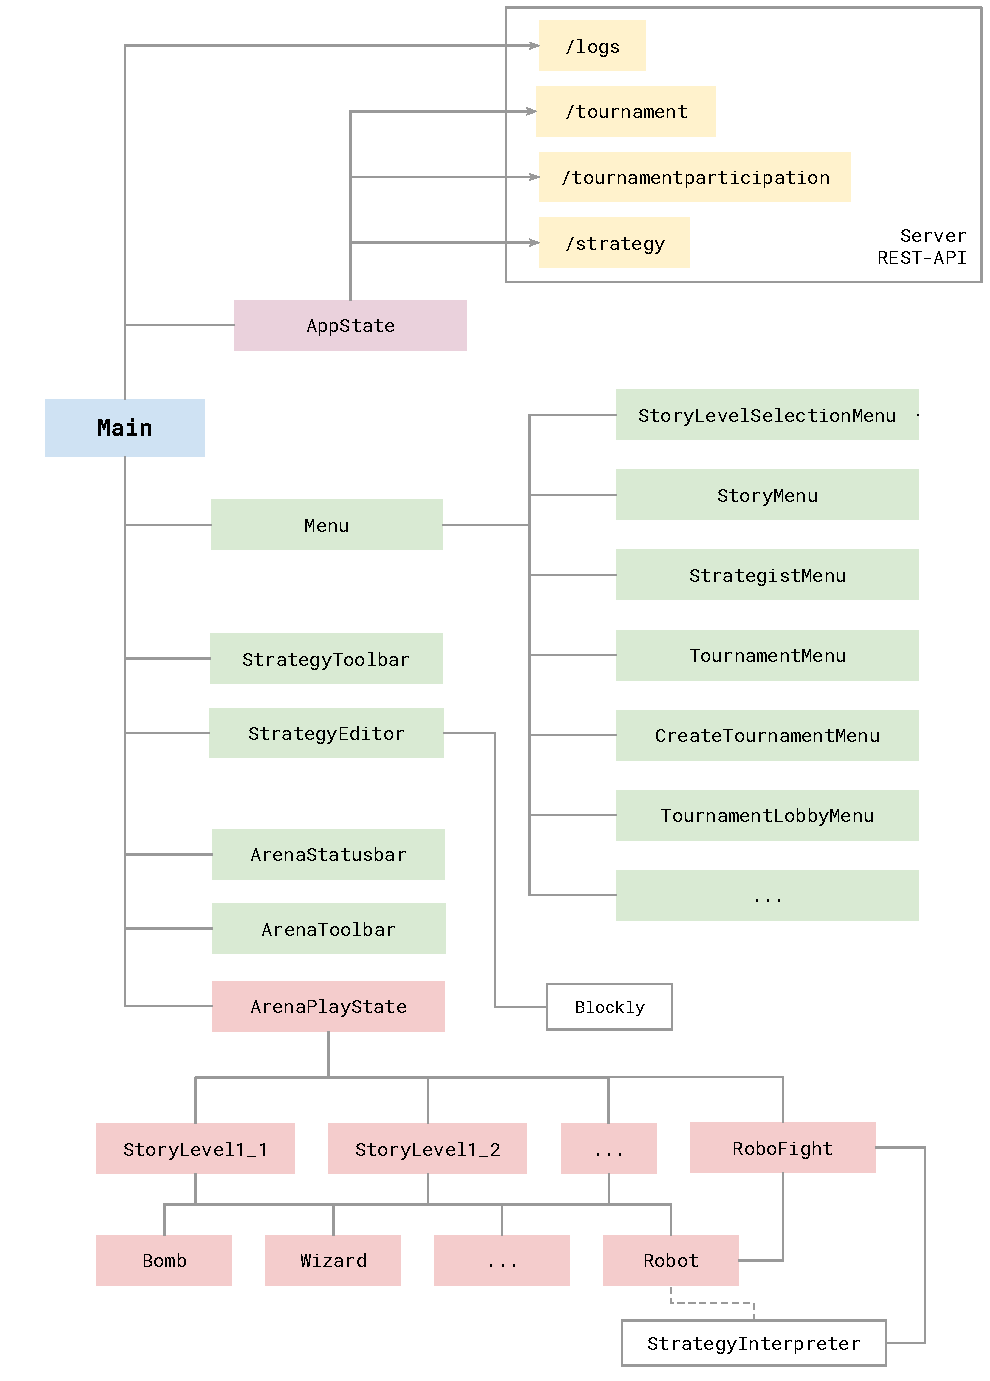
\includegraphics{figures/architektur.pdf}
\end{figure}

Einzelne Komponenten wurden in native Javascript-Module übersetzt. Nun werden Abhängigkeiten
zwischen Modulen über import-Statements explizit ausgedrückt. Anstatt alles auf einen globalen
Namespace zu legen, definieren Module über export-Statements explizit, welche Variablen, Funktionen
oder Klassen von anderen Modulen importiert werden können. Dies erhöht die Sichtbarkeit von
Abhängkeiten und damit die Wartbarkeit des Programms beträchtlich. Es verhindert zudem, dass interne
Variablen einer Komponente von anderen Komponenten benutzt oder verändert werden.

Das ctGameStudio mit Open Stage-Modus braucht die Möglichkeit, aufgrund des Programmzustands
HTML-Komponenten dynamisch darzustellen. Mithilfe der
hyperHTML\footnote{https://viperhtml.js.org/}-Bibliothek wurden Komponenten konzipiert, die ineinander
verschachtelt werden können, deren HTML und Event-Listener deklarativ ausgedrückt werden, und
effizient gerendert und aktualisiert werden können.

\subsection{Main}

Der Hauptfunktion kommt nun eine größere Rolle zu. Während in der Erstversion lediglich die
Initialisiation des Strategieeditors und der Arena stattfand, und die Komponenten direkt aufeinander
zugriffen, findet in diesem Top-Level-Modul nun die Koordination aller Komponenten statt. Kern
dieser Koordination ein Modell des Programmzustands.

Als Programmzustand werden hier die Parameter bezeichnet, die bestimmen, welche Komponenten
gerendert werden und welche Daten diese darstellen. In der App wird er durch ein unveränderliches
Javascript-Objekt modelliert (Abb. \ref{state-model} zeigt einen beispielhaften Ausschnitt aus dem
Zustandsobjekt, das Zustande kommt, wenn der Nutzer zu der Liste von seinen Turnieren navigiert). Das
Zustandsobjekt ist unveränderlich (\enquote{Immutable}), so dass sein Inhalt nie direkt im Speicher
geändert werden kann. Soll der Zustand geändert werden, muss eine Kopie dessen angelegt werden.
Dieser Schutz sorgt dafür, dass keine Komponente, die eine Referenz auf den Zustand hat, diesen
direkt für andere Komponenten ändern kann.

Änderungen des Zustands finden ausschließlich im Main-Modul statt, und müssen von Komponenten
explizit über das versenden von \enquote{Actions} herbeigeführt werden (Abb.
\ref{update-loop-diagram}). Die Update-Funktion (Abb. \ref{update-loop}) ist dafür zuständig,
aufgrund einer Action einen neuen Zustand zu bauen. Auf die Aktualisierung des Zustands folgt die
Darstellung des neuen Zustands mithilfe der Render-Funktion. Sie erhält den Programmzustand und gibt
einr Struktur aus hyperHTML-Elementen zurück. Mithilfe von hyperHTML wird diese in das DOM
eingefügt. Bei wiederholter Darstellung der Struktur aufgrund von Veränderungen des Zustands nimmt
die Bibliothek nur die minimalen Änderungen am DOM vor, die nötig sind, um die veränderte Struktur
darzustellen. So ist es möglich, die Render-Funktion bei jeder Zustandsaktualisierung komplett
auszuführen, ohne das DOM dabei komplett neu zu konstruieren und durch den Browser darzustellen.
Dadurch wird vermieden, in der Darstellungsebene komplizierte Logik zu brauchen, die bestimmt, wann
und wie das DOM geändert wird.

Dieses System ist dazu konzipiert, keine unvorgesehenen oder schlecht nachvollziehbaren Änderungen
des Programmzustands zu haben. Durch die explizite Änderung durch Actions ist immer sichtbar, wann
und wie sich der Zustand verändert hat. Die Business- und Darstellungs-Logik ist in zustandslosen
und damit einfach zu testenden Funktionen hinterlegt (Update- und Render-Funktion). Bei
Programmfehlern ist leicht nachvollziehbar, ob der Fehler in der Darstellung liegt, oder ob ein
unkorrekter Zustand gebildet wurde. Durch die explizite Modellierung des Zustands, der Actions und
der Aktualisierung des Zustands in Form der Update-Funktion ist übersichtlich zu sehen, welche
Formen der Zustand annehmen kann.


\begin{figure}
  \caption{Ausschnitt aus dem Zustandsmodell.}

  \label{state-model}

  \begin{lstlisting}
{
  view: VIEW_MENU,
  currentMenu: MENU_TOURNAMENT_LIST,
  tournamentsList: {
    isLoading: false,
    success: true,
    tournaments: [
      {
        "_id":"xxxxx",
        "accessCode": "1OVkM",
        "createdBy": "5acf147740f1e526a82c21ea",
        "publishedDate": "2018-07-29T18:55:16.995Z",
        "maxMatchDuration": 120,
        "maxRoundCount": 1,
        "mode":"TOURNAMENT_MODE_ROUND_ROBIN",
      },
      ...
    ]
  },
  ...
}
  \end{lstlisting}
\end{figure}

\begin{figure}
  \caption{Darstellung und Aktualisierung des Spiels.}

  \label{update-loop-diagram}
  
  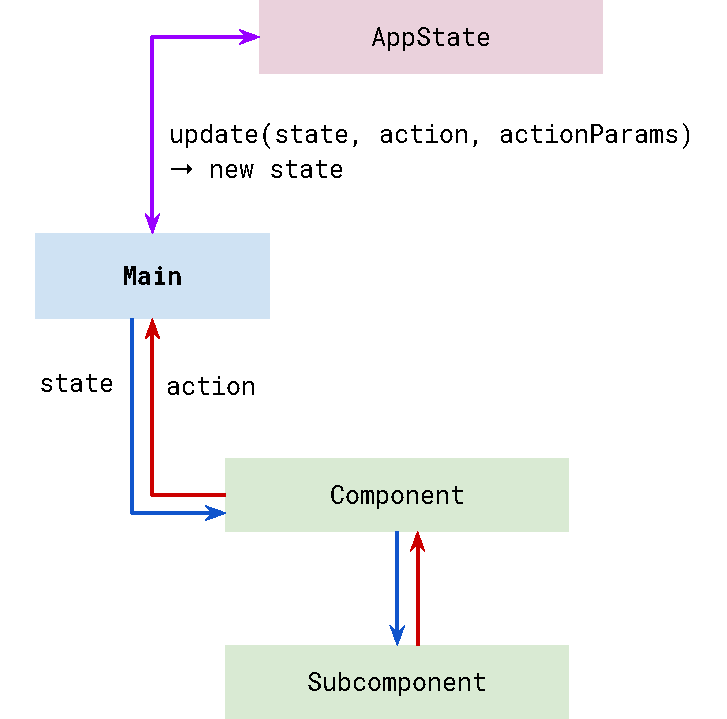
\includegraphics{figures/statemanagement-flow.pdf}
\end{figure}

\begin{figure}
  \caption{Vereinfachter Auszug des Codes zur Darstellung und Aktualisierung des Spiels.}

  \label{update-loop}

  \begin{lstlisting}
  let state;
  let root = document.querySelector('#app');
  let menuComponent = new MenuComponent();
  let arenaComponent = new ArenaComponent();
  let editorComponent = new StrategyEditorComponent();

  root.addEventListener(
    'update', // custom event
    (event) => handleAction(event.detail.name, event.detail.params)
  );

  handleAction(ACTION_INITIALIZE);

  function handleAction (action, params) {
    state = update(state, action, params);
    hyperHTML.bind(root, render(state));
  }

  function render (state) {
    if (state.viewMode === VIEW_MENU) {
      return hyperHTML.wire()`
        <div class="menu">
          ${menuComponent.render(state)}</div>
          <button onclick=${() => 
            this.dispatch('action', { type: ACTION_MENU_BACK })
          }>Back</button>
        `;
    } else if (state.viewMode === VIEW_TRAINING) {
      return hyperHTML.wire()`
        <div class="editor">${editorComponent.render(state)}</div>
        <div class="arena">${arenaComponent.render(state)}</div>`;
    } else if (state.viewMode === VIEW_TOURNAMENT) {
      ...
  }

  function update (state, action, params) {
    switch (action) {
      case ACTION_INITIALIZE: return initialState;
      case ACTION_OPEN_STORY_MENU:
        return state.set('currentMenu', MENU_STORY);
      ...
    }
  }
  \end{lstlisting}
\end{figure}

Das beschriebene Zustandsmanagement lässt sich nicht auf Phaser übertragen. Wie in Abschnitt
\ref{arena-alt} beschrieben, arbeitet Phaser mit regulären, veränderbaren Javascript-Objekten und
einem eigenen Update/Render-Loop. Daher wird die Arena-Komponente nicht bei jeder Aktion neu
dargestellt, sondern bei Start des Trainings oder Start eines Turnierkampfes einmalig initialisiert.
Zustand, der sowohl die Arena als auch den Rest des Spiels betrifft, ist doppelt im System
repräsentiert; einmal im Programmzustand und einmal in den Spielobjekten der Arena. Über ein
Event-Interface der Arena-Komponente werden die beiden Zustände synchronisiert. Ein Beispiel soll
anhand der Lebenspunktzahl der Roboter gegeben werden. Einerseits wird sie im Roboter-Spielobjekt
des Roboters gespeichert und bei Treffern verändert. Andererseits wird auch im Programmzustand
dieser Wert gespeichert, um die Lebenspunkte in der Statusbar, die eine HTML-Komponente ist,
anzuzeigen. Um die Werte zu synchroniesieren, wird bei Treffer eines Roboters ein Ereignis
ausgelöst. Dieses Ereignis wird in eine Aktion transformiert, die dann den Programmzustand ändert.


\subsection{Datenpersistenz}

Der ctGameStudio-Server unterstützt MongoDB für die Persistenz von Daten. Mithilfe von KeystoneJS
werden JSON-Rest-APIs bereit gestellt, über die Daten gespeichert und geladen werden. Dazu können
Schemas definiert werden, die die Struktur und Datentypen eines Modells festlegen, und zur
Validation der Daten benutzt werden.

In der Erstversion des ctGameStudio bereits verfügbar war das Nutzermanagement, welches das Einloggen und
Personalisieren der der Spielinhalte ermöglicht, und eine JSON-Rest-Endpunkt zum Loggen von
Spielereignissen zur späteren Nachbereitung. Um den Open Stage-Modus zu unterstützen, mussten neue
Endpunkte und Datenmodelle für Strategien, Turniere und Teilnahmen an Turnieren erstellt werden.

Im ctGameStudio mit Open Stage-Modus werden Server-Anfragen werden durch Actions angestoßen, und im
AppState-Modul abgehandelt. Nach der Antwort durch den Server werden wiederrum Actions angestoßen,
um das User Interface zu aktualisieren. Dabei wird das Anfrageergebnis und der Anfragestatus im
Programmzustand gespeichert. Dazu gehört die Information, ob die Anfrage gestartet wurde, ob sie
abgeschlossen wurde, und ob sie erfolgreich oder fehlerhaft war. Diese Informationen werden benutzt,
um im Dialog entsprechendes Feedback an den Nutzer zu geben.

Abb. \ref{create-tournament-flow} stellt beispielhaft den Prozess dar, der beim Erstellen eines
neuen Turniers abläuft. Aufgrund des initialen Zustands zeigt der Dialog das Turnierformular an
(Schritt 1). Wenn der Nutzer den Button zur Erstellung des Turniers drückt, wird eine Aktion zum
Starten der Anfrage ausgelöst (Schritt 2). Als Aktionsparamter werden die Turnieroptionen beigefügt,
die der Nutzer eingestellt hat. Im Hintergrund wird die an den Turnier-Endpunkt mit den übergebenen
Parametern gestartet. Der Dialog zeigt nun an, dass die Anfrage läuft. War das Speichern erfolgreich
(Schritt 3a) wird der Programmzustand über eine entsprechende
Action wird der Programmzustand aktualisiert, um dem Nutzer nun Feedback über das erfolgreiche
Speichern zu geben, und den vom Server generierten Zugangscode anzeigen. Trat bei der Anfrage ein
Fehler auf (Schritt 3b), wird über eine andere Action ausgelöst, welche den Programmzustand um die
Fehlerinformation bereichert. Daraufhin kann im Dialog eine entsprechende Fehlermeldung angezeigt
werden.
 
\begin{figure}
  \caption{Verlauf von Actions und dem Programmzustand beim Speichern eines Turnieres.}

  \label{create-tournament-flow}

  \begin{lstlisting}
  1) Öffnen des Dialogs

     -> Programmzustand: {
       requestStarted: false
     }

  2) Action: CREATE_TOURNAMENT_REQUEST,
     Parameter: { maxRoundDuration: 3, maxRoundCount: 1, ... }

     -> Anfrage: POST /tournament

     -> Programmzustand: {
       requestStarted: true,
       isLoading: true
     }

  3a) Action: CREATE_TOURNAMENT_SUCCESS
       Parameter: { accessCode: 'xxxxxx' }

     -> Programmzustand: {
       requestStarted: true,
       isLoading: false,
       success: true,
       accessCode: 'xxxxxx'
     }

  3b) Action: CREATE_TOURNAMENT_FAILURE

     -> Programmzustand: {
       requestStarted: true,
       isLoading: false,
       success: false,
       failureReason: UNEXPECTED_SERVER_ERROR
     }
  \end{lstlisting}
\end{figure}


\subsection{Strategieinterpreter}

In der Erstversion des ctGameStudio wurde die Schritt-Funktion des Strategie-Interpreters aus drei Komponenten
aufgerufen - bei erster Ausführung der Strategie durch die Toolbar, bei Beenden einer Aktion aus dem
Roboter, und aus der Update-Funktion des PlayState. Dieser Aufbau stellte unnötige Komplexität dar,
und machte es schwer zu identifieren, wann genau die Schrittfunktion aufgerufen wird. Die Einführung
einer zweiten, parallel ausgeführten Strategie durch den Open Stage-Modus motivierte eine
Vereinfachung der Strategieausführung.

Im ctGameStudio mit Open State-Modus wird der StrategieInterpreter nur aus dem PlayState heraus
aufgerufen (Abb. \ref{strategy-interpreter-new}). Die Schrittfunktionen der Interpreter der beiden
Strategien werden kontinuierlich bei jedem Update ausgeführt. Dadurch wird auch der Aufruf aus der
Roboter-Klasse hinfällig.

Um zu vermeiden, dass die Ausführung der Strategie bis zur nächsten Unterbrechung zu lange dauert,
und es dazu zu Framedrops kommt, als auch die Ausführung der Aktionen des Gegner-Roboters verschoben
wird, wird die Ausführung auf eine geringe Zeit begrenzt. Um Stack Overflows vorzubeugen, wird die
wiederholte Ausführung der Schritt-Funktion des JS-Interpreters mit einer while-Schleife realisiert.


\begin{figure}
  \caption{Vereinfachter Auszug aus dem PlayState und dem StrategyInterpreter, der die vereinfachte
  Strategieausführung verdeutlicht.}

  \label{strategy-interpreter-new}

  \begin{lstlisting}
    // PlayState
    function create () {
      ...
      player1Interpreter = StrategyInterpreter(
        player1StrategyCode, player1Robot
      );
      player2Interpreter = StrategyInterpreter(
        player2StrategyCode, player2Robot
      );
      ...
    }

    function update () {
      ...
      player1Interpreter.executeNextCommand();
      player2Interpreter.executeNextCommand();
      ...
    }

    // StrategyInterpreter
    ...
    function executeNextCommand() {
      if (!robot.isIdle || !robot.sprite.alive) {
        return;
      }
      const lastReturnTimestamp = Date.now();
      let hasMoreCode = interpreter.step();
      while (
        hasMoreCode &&
        robot.isIdle &&
        robot.sprite.alive &&
        Date.now() - lastReturnTimestamp <= MAX_TIME_SPENT_IN_EXECUTION
      ) {
        hasMoreCode = interpreter.step();
      }
    }
    ...
  \end{lstlisting}
\end{figure}


\section{Anpassung des Roboterkampfes}

Da sich nun zwei Roboter auf dem Spielfeld befinden, musste entschieden werden, was bei Kollisionen
zwischen diesen Robotern passiert. Um die Strategien in diesem Fall möglichst uneingeschränkt weiter
laufen zu lassen, stoßen sich die die Roboter bei einer Berührung voneinander ab, und setzen ihre
Bewegung fort. Umgesetzt wurde dies mit der Standard-Kollisionsfunktion der Phaser-Arcade-Physik
\ref{https://photonstorm.github.io/phaser-ce/Phaser.Physics.Arcade.html#collide}.

Um die Evaluation seitens des Strategieentwicklers zu unterstützen, ist es sinnvoll, Roboteraktionen
in einem langsamen, gut nachverfolgbaren Tempo auszuführen. Dabei soll das Gameplay spannend
bleiben. Da die Geschwindigkeit der Roboteraktionen als zu schnell empfunden wurden, wurden
relevante Konstanten und Timingberechnungen in der Roboter-Klasse angepasst, um die Bewegungs- und
Drehgeschwindigkeit der Roboter sowie die Geschwindigkeit der Schussprojektile zu verringern.

Um Ausweichmanöver ermöglichen zu können, wurde die Scanfähigkeit eingeschränkt. Ein Ausweichmanöver
besteht darin, seine Position zu verändern, nachdem man festgestellt hat, dass man getroffen wurde.
Wenn der Gegner in einer Schleife dauerhaft auf einen Schuss direkt einen Scanvorgang folgen lässt,
kann er jedoch jede Bewegung nachverfolgen. Ausweichen nach Treffern war so kaum möglich. Der
Scanvorgang wurde daher so angepasst, dass er nicht mehr verzögerungsfrei über das gesamte
Spielfeld reicht. Stattdessen muss sich der Scanstrahl nach einer Bewegung oder einem Schuss nun
erst ausbreiten, bis er seine volle Reichweite erreicht hat. Ein Scan von der einen Spielfeldseite
bis zur Anderen dauert nun wenige Sekunden. Um dem Strategieentwickler Kontrolle über die Dauer des Scans
zu geben, wurde der Scanblock um einen Parameter erweitert, mit dem die maximale Reichweite
angegeben werden kann, die erreicht werden soll, bis der nächste Block ausgeführt wird.

Zur Implementation dieser Änderung wurde die Roboter-Klasse und die Scanblöcke angepasst. Die
Scan-Methode hatte zuvor den gesamten Scanvorgang behandelt, und hatte das Scanergebnis als
Rückgabewert. Nun initialisiert sie den Scanvorgang lediglich, und gibt ein Objekt zurück, das erst
nach Abschluss des Scans das Scanergebnis beinhaltet. Die Update-Funktion der Roboter-Klasse wurde
erweitert, so dass der Scanstrahl aufgrund seiner Ausbreitung über die Zeit kontinuierlich neu
dargestellet wird, kontinuierlich festgestellt wird, ob ein Gegner durch den Strahl erfasst wurde,
und der Scanvorgang beendet wird, wenn ein Roboter erfasst wurde, oder der Rand des Spielfelds, bzw.
die angegebene Scanreichweite erreicht wurde. Der Code, der aus den Blöcken generiert wird, die mit
dem Scanergebnis arbeiten, wurde angepasst, um mit dem Objekt arbeiten zu können, dass von der
Scan-Methode zurück gegeben wird.


\section{Turnierausführung}

TODO
% Zu Beginn der Ausführung eines Turniers wird die Matchstruktur kalkuliert. Bei einem Turnier
% Jeder-gegen-Jeden (engl. round robin) werden dazu Paare aus 


